\section{Chrome extension architecture}
\label{sec:ExtDetails}
As already discussed before, a Chrome extension is a software that extends the potentiality of the browser and enhances the user experience. Such extensions are not stand-alone software, but are integrated in the browser. The integration is done through a powerful API that expose to the developer lots of functionality of the browser. Since Chrome extensions interact with web pages and with browser them are developed using the classic web-style language: JavaScript. Extension can have even HTML or CSS files and can contains various resources that can be either local or remote resources as typical in the web.

As showed in \cite{ChromeExtensionOnline} a Chrome Extension is an archive containing files of various kind like JavaScript, HTML, JSON, images and others that extends the browser features.

A basic extension is composed by a manifest file and one or more JavaScript or Html files.

\subsection{Manifest}
The manifest file \texttt{manifest.json} is a JSON-formatted file. It contains all the specification of the extension and for this reason is the entry-point of the extension. Indeed when an extension is load, the loader finds the manifest file and from it create the components of the extension. It contains two mandatory fields: \texttt{name} and \texttt{version} respectively containing the name and the version of the extension. Other important fields are:
\begin{itemize}
\item \texttt{background}: contains an object with either \texttt{script} or \texttt{page} field. The former contains the source of the content script, while the other the source of an HTML page. If the \texttt{script} field is used, the scripts are injected in a empty extension core page, while if it is used \texttt{page} the HTML document with all its elements (e.g., scripts) composes the extension core;
\item \texttt{content\_scripts}: contains a list of content script objects. Each object contains the field \texttt{matches}, a list of match patterns (Match patterns are explained below), and a field \texttt{js} containing the list of JavaScript source files to be injected;
\item \texttt{permissions}: contains a list of privileges that are requested by the extension. These can be either a host match pattern for XHR request or the name of the API needed.
\end{itemize}

Another possible field is \texttt{optional\_permissions}. It contains the list of optional permissions that the extension could require. It is used to restrict the privileges granted to the app. To use one of this permissions the background page has to explicitly require it and, after having used it, the permission has to be released. A program using the optional permissions can reduce the possible privileges escalated by an attacker.

A match pattern is a string composed of three parts: \texttt{scheme}, \texttt{host} and \texttt{path}. Each part can contain a value, or \texttt{"*"} that means all possible values. In table \ref{tab:URLPatSyn} is shown the syntax of the URL patterns; more details are reported in \cite{ChromeExtensionMatch}. In this way we can decide to inject some content scripts only on pages derived from a given match. This is used when a content script of the extension has to interact with only certain pages. For example \texttt{"*://*/*"} means all pages; \texttt{"https://*/*"} means all HTTPS pages; \texttt{"https://*.google.com/*"} means all HTTPS domains that are subdomains of google with all their possible path (e.g., \texttt{mail.google.com}, \texttt{www.google.com}, \texttt{docs.google.com/mine/index.html}).

\begin{table}[tlb]
\begin{verbatim}
<url-pattern> := <scheme>://<host><path>
<scheme> := '*' | 'http' | 'https' | 'file' | 'ftp' | 'chrome-extension'
<host> := '*' | '*.' <any char except '/' and '*'>+
<path> := '/' <any chars>
\end{verbatim}
\caption{Url pattern syntax. Table taken from \cite{ChromeExtensionMatch}}
\label{tab:URLPatSyn}
\end{table}

In table \ref{src:AManifest} we can see a manifest of a simple Chrome extension that expands the feature of moodle. We can see that the extension has an empty background page on which the file \texttt{background.js} is injected. It also has permissions \texttt{tabs} and \texttt{download}, and can execute XHR to pages with every path in \texttt{https://moodle.dsi.unive.it/}. It has also one content script that is injected in all subpages of \texttt{https://moodle.dsi.unive.it/}.
\begin{table}[tlb]
\lstset{language=java,showstringspaces=false}
\begin{small}
\begin{lstlisting}
{
	"manifest_version": 2,
	"name":"Moodle expander",
	"description":"Download homework and uploads marks from a JSON string",
	"version":"1",
	"background": { "scripts": ["background.js"] },
	"permissions":  
		[
			"tabs",
			"downloads",
			"https://moodle.dsi.unive.it/*"
		],
	"content_scripts": 
		[
			{
				"matches": ["https://moodle.dsi.unive.it/*"],
				"js": ["myscript.js"]
			}
		]
}
\end{lstlisting}
\end{small}
\caption{A manifest file}
\label{src:AManifest}
\end{table}

\subsection{Content scripts}
Content scripts are JavaScript source files that are automatically injected to the web page if this matches with the pattern defined in the manifest. Otherwise it can be programmatically injected by a background page using the \texttt{chrome.tabs.executeScript} call (the function requires \texttt{tabs} permission). In the example of table \ref{tab:URLPatSyn} the JavaScript file \texttt{myscript.js} is injected to all sub-pages of \texttt{https://moodle.dsi.unive.it/}. In the extension framework content scripts are designed to interact with pages. Since this interaction could be the entry point for an attacker, content scripts have no permissions except the one used to communicate with the extension core. In order to reduce injection of code in the content script from a malign page, there is a strong isolation between the heaps of these two. Content scripts of the same extension are run together in their own address space, and the only way they have to interact with the page on which they are injected is via the DOM API. DOM API lets the content scripts access and modify only standard fields of the DOM object, while other changes are kept locally\cite{ChromeExtSpec}. This strong isolation mitigate the risk of code injection since it blocks almost completely pointer exchange. In figure \ref{fig:SepWorlds} is showed such relation.

\begin{figure}[htb]
    \centering
    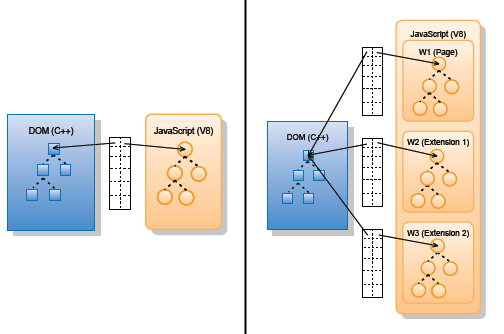
\includegraphics[scale=1]{Both}
    \caption{On the left the normal one-to-one relation between DOM implementation and JavaScript representation; On the right the one-to-many relation caused by running content scripts in isolated worlds. Figure taken from \cite{ChromeExtSpec}}
    \label{fig:SepWorlds}
\end{figure}

In order to keep functionality of extensions, communication between content scripts and extension core is done using a message passing interface. The message passing interface has crucial importance in this work since it is the only way for a content script to trigger execution of a privilege. We will discuss it later in \ref{subs:MPI}.

\subsection{Extension core}
The extension core is the most critical part of the application. It is executed in a unique origin like \texttt{chrome-extension://hcdmlbjlcojpbbinplfgbjodclfijhce} in order to prevent cross origin attacks, but it can communicate with all origins that match with one of the host permission defined in the manifest. In this environment are executed all scripts defined in the background field of the manifest. Since background pages can have remote resources of every kind (even scripts), they can also request to the web such resources, but this can be very dangerous. In fact if the resources are on HTTP connections these can be altered by an attacker. \cite{ChromeExtSpecSnd} describes how to enforce the security policy in order to avoid such possible weakness. Background pages can interact with content scripts via message passing.
%\missingfigure{Maybe figura schema Chrome Extensions comm \& elements.}

\subsection{Message passing API}
\label{subs:MPI}
Every content script of the extension can use the message passing interface. To do this it has to use the functions contained in the \texttt{chrome.runtime} object \cite{ChromeExtensionRuntime} that exposes such API.

The main way to send a message to the extension core is invoking the method \texttt{chrome.runtime.sendMessage}. Like all Chrome APIs even the message passing is asynchronous. As primary arguments it takes the message that can be of any kind and a callback function that is triggered if someone answer to the message. Before sending, the message is marshaled using a JSON serializer.

In order to listen to incoming messages, a component has to register a function on the \texttt{chrome.runtime.onMessage} event. This function will be triggered when a message arrives. Its arguments are the message (unmarshalled by the API), the sender and an optional callback used to send response to the sender of the message. The sender field is very important because it is the only way to know the real identity of the sender. In fact the message may not be used to decide the sender, because it can be of every kind.

Since content scripts are multiple and injected in various pages (tabs), the extension core for sending a message has to use the \texttt{sendMessage} method of the \texttt{tab} object to which the message has to be sent. Its behavior is the same of the \texttt{chrome.runtime.sendMessage} method.

In table \ref{tab:MPIMessage} we can see how to use the simple message passing interface. A component simply sends the message and wait for a response. The other registers \texttt{onMessage} function in the event listener \texttt{onMessage}. When the handler is triggered by an incoming message \texttt{onMessage} function it checks the message and decides to compute something according to the request or refuses the message doing nothing.

Another way to communicate, that is more secure, is using channels as in table \ref{tab:MPIPort}. In the message passing API there is a method called \texttt{connect} that triggers the corresponding event listener \texttt{onConnect} and returns a port. It has as optional arguments the name of the channel that is creating. A port object is a bidirectional channel that can be used to communicate. It contains the methods \texttt{postMessage}, \texttt{disconnect} and the events \texttt{onMessage} and \texttt{onDisconnect}. Communication using ports instead of the classical \texttt{chrome.runtime.sendMessage} is more secure, because only who has one of the port endpoint can communicate. Obviously ports are not serializable, so it is impossible to leak the ownership of a port. Ports provide a guarantee for the sender of the message.

\lstset{language=java,showstringspaces=false}
\begin{table}[htb]
\begin{small}
\begin{center}
\begin{tabular}{p{0.45\linewidth} | p{0.45\linewidth}}
Sender & Receiver\\
\hline
\begin{lstlisting} 
var info = "hello";
var callback = 
	function(response) 
	{ 
		console.log("get response: " + response);
	};
chrome.runtime.sendMessage(info, callback);
\end{lstlisting}&
\begin{lstlisting} 
var onMessage = 
	function(message, sender, sendResponse) 
	{ 
		if (message = "hello") 
		{
		    //compute message
			sendResponse("hi");
		}
		else 
			console.log("connection refused from"+sender);
	};
chrome.runtime.onMessage.addListener(onMessage);
\end{lstlisting}\\
\end{tabular}
\end{center}
\end{small}
\caption{Sending a message.}
\label{tab:MPIMessage}
\end{table}

\begin{table}[htb]
\begin{small}
\begin{center}
\begin{tabular}{p{0.45\linewidth} | p{0.45\linewidth}}
Port opening active & Port opening passive\\
\hline
\begin{lstlisting} 
var port = chrome.runtime.connect({name: "cs1"});
port.onMessage.addListener(onMessage)
port.postMessage("hi")
\end{lstlisting}&
\begin{lstlisting} 
var scriptPort = null;
var onConnect = 
	function(port) 
	{ 
		if (port.name = "cs1") 
		{
			scriptPort = port;
			port.onMessage.addListener(onMessage);
		} 
		else 
		{
			console.log("connection refused"); 
			port.disconnect();
		}
	};
chrome.runtime.onConnect.addListener(onConnect)
\end{lstlisting}\\
\end{tabular}
\end{center}
\end{small}
\caption{Port creation.}
\label{tab:MPIPort}
\end{table}

\section{Permission bundling}
\label{sec:BundlingExample}
Modern privilege-separated architectures mitigates various attacks coming from the external untrusted world, but they still have weakness. A great part of this weakness derive from bad-practice of developers that often are not security experts. One of this is called bundling. Bundling is, as the name suggests, the practice of clustering in the same component different privileges. This can be very dangerous because an attacker that compromise the bundled component can escalate all privileges clustered in it. 

In Chrome extensions sometimes programmers tend to aggregate in a single function various privileges that are delegated to different components. Moreover, often, the bundled function is the \texttt{onMessage} listener in the background, that is the entry point for an attacker that has compromised a content script. The \texttt{onMessage} function is, indeed, critical because it receives  messages from a possible compromised content script, since attacker cannot access directly the background page from the web thanks to the privilege separated and strong isolation behavior of the architecture. The practice of permission bundling, especially in the \texttt{onMessage} function is very dangerous because an attacker that compromises a content script can directly trigger the listener in order to escalate privileges. 

To reduce the attack surface exposed by bundled components, is important to base the decision of which privilege has to be exercised on trusted elements. Indeed, as seen in table \ref{tab:MPIMessage}, the choice taken by the bundled component when a message is received can depend on various factors decided by the programmer.

Let us explain the example in \ref{tab:Bundled}: suppose to have three components Background, CS1 and CS2. CS1 can only send messages that has \texttt{"getPasswd"} as title and CS2 only \texttt{"executeXHR"}. Here the Background deduct the sender checking the title of the messages instead of of explicitly checking the argument \texttt{sender}. According to the check decides which privilege has to be executed. This practice exposes all the weakness of the bundling and is very dangerous because an attacker can compromise just one of the two content scripts and from that one can forge messages with any form to escalate a permission that it does not have in the original setting.

To mitigate such weakness, in chrome extensions, is important to check the sender field of the \texttt{onMessage} function in order to be sure of the sender. This cannot be enough because, as discussed before, contents script that are injected on the same page share their memory, tab and origin, and the message passing interface are does not distinguish them. The fix of this weakness is to use ports instead of the \texttt{chrome.runtime.sendMessage} function in order to have different listener for each content script. In this way we unbundle the \texttt{onMessage} function, separating in the various listeners privileges. In table \ref{tab:UnBundled} are showed a not dangerous bundled code, and an unbundled code.

\begin{table}[htb]
\begin{small}
\begin{center}
\begin{tabular}{p{0.95\linewidth}}
Background\\
\hline
\begin{lstlisting}
function onMessage(message, sender, response)
{    	
	switch (message.title) {
		/* Requests from content script 1 */
		case "getPasswd":
		// get passwords
		response(passwd)
		break;
		
		/* Requests from content script 2 */
		case "executeXHR":
		var host = message.host
		var m = message.content;
		// execute XHR on args
		break;
				
		default:
		throw "Invalid request from contentScript";
	}
}
\end{lstlisting}\\
\hline
\hline
Content script CS1 \\
\hline
\begin{lstlisting}
var mess = {title: "getPasswd"};
chrome.runtime.sendMessage(mess);
\end{lstlisting}\\
\hline
\hline
Content script CS2\\
\hline
\begin{lstlisting}
var mess = {title: "executeXHR", host: "www.google.com", content: "hi there"};
chrome.runtime.sendMessage(mess);
\end{lstlisting}\\
\end{tabular}
\end{center}
\end{small}
\caption{Bundled code.}
\label{tab:Bundled}
\end{table}
\begin{table}[htb]
\begin{small}
\begin{center}
\begin{tabular}{p{0.95\linewidth}}
Unbundling checking sender\\
\hline
\begin{lstlisting}
function onMessage(message, sender, response)
{    	
	switch (sender) {
		/* Requests from content script 1 */
		case CS1:
		// get passwords
		response(passwd)
		break;
		
		/* Requests from content script 2 */
		case CS2:
		var host = message.host
		var m = message.content;
		// execute XHR on args
		break;
				
		default:
		throw "Invalid request from contentScript";
	}
}
\end{lstlisting}\\
\hline
\hline
Unbundling using ports.\\
\hline
\begin{lstlisting}
// Handler for messages from CS1
function onMessage_cs1(message, sender, response)
{    	
	/* Requests is content script 1 since it is on its port */
	// get passwords
	response(passwd)
}
// Handler for messages from CS2
function onMessage_cs2(message, sender, response)
{    	
	/* Requests is content script 2 since it is on its port */
	var host = message.host
	var m = message.content;
	// execute XHR on args
}
port_cs1.onMessage.addListener(onMessage_cs1);
port_cs2.onMessage.addListener(onMessage_cs2);
\end{lstlisting}\\
\hline
\end{tabular}
\end{center}
\end{small}
\caption{Unbundling.}
\label{tab:UnBundled}
\end{table}

%The existence of the undefined value and im-
%plicit type coercions in the language means that even minor
%spelling errors, for example in a property name, often has
%surprising consequences at runtime. With statically typed
%languages, the type systems provide a strong foundation for
%detecting such errors. In contrast, because of the dynamic
%nature of JavaScript web application code, our analysis must
%be capable of reasoning about the flow of control and data
%throughout the applications.

\section{Flow logic}
\label{sec:FlowLogic}
The goal of this work is to develop an analysis that is able to detect statically absence of bundling in real Chrome extensions. Moreover we want to do this automatically, so without any effort for the developer (e.g., code annotations or similar). Statically typed languages are easier to check because the typing discipline provide strong foundation for detecting the behavior of a program. On the contrary, the weak dynamically typed nature of JavaScript code makes the analysis more difficult. Since extension are written in JavaScript we have to face with problem deriving from a dynamic and weak typing discipline. Indeed, in JavaScript there are lots of quirks that made the analysis very hard with a classical typing approach. For example local and global scoping, passage of functions, and access of a property of an object using a string are very hard to handle statically. To achieve our purpose the analysis must track the flow of both control and data during the execution. In this scenario we used the flow logic approach because of its flexibility, high potential and easiness to use.

Flow logic, introduced in \cite{FlowLogic}, is a static analysis approach that derives from state of the art in program verification and has been successfully used in research projects \cite{CarmelFlowLogic,CarmelFlowLogicFormalization}. It has its root in classical approaches of static program analysis \cite{PrincipleProgramAnalysis} like control flow analysis \cite{CMLCFA}, abstract interpretation, constraint based analysis and data flow analysis. Flow logic lets the specification to focus on when an analysis estimate is acceptable, instead of how to compute such estimate. Another property is that, like structural operational semantics, is adaptable to lots of programming paradigms. Finally it can be used with various levels of abstraction according to the implementation details that are needed, but can be easily translated from one level to another. 

The principal levels of abstraction are grouped in some possible approaches: abstract versus compositional and succinct versus verbose. The abstract style is closer to standard semantics while the compositional one is more syntax directed. The succinct approach is similar to the typical style of type systems because it focuses the top part of the analysis, while the verbose approach traces all the internal information in cashes and are typical of the implementation of control flow analysis and constraint based analysis.

The modularity fits very well for analysis, because the abstract succinct style is very clean and expressive without dealing with implementation details, and from such specification is easy to commute it to a compositional verbose specification. From the latter is possible to build an algorithm for generating the set of constraints of a program and combining it with a simple constraint solver like the worklist algorithm \cite{PrincipleProgramAnalysis} or with a more sophisticated ones like the succinct solver \cite{SuccinctSolver} or the BANSHEE solver \cite{BansheeSolver}, is possible to compute the estimate for a program.

Let us have an example: suppose to have a program and ``magically'' an estimate for it: using flow logic judgments we are able to establish if such estimate respect our analysis for the program, or not. This decision is granted by the fact that one of the constraint of generated by the constraint generator is not satisfied. Moreover we can compute starting from the constraint an estimate that satisfy the analysis.

In this work, is used the flow logic, and as described before, the various specification-to-implementation steps are done. In chapter \ref{chap:Formalization} is used an abstract-succinct approach, and in chapter \ref{chap:Implementation} the analysis is expanded in the compositional-verbose one; from this the algorithm for constraint-generation is built and finally is used a worklist algorithm to solve the constraints and to find an estimate for a program.

\section{Lambda JS}
Since JavaScript is a real world programming language that has high level constructs, weak and dynamic typing discipline and unconventional semantics, it is very complex to analyze. We reduce JavaScript to \ljs\ as described in \cite{LambdaJS}. \ljs\ is a dialect of Scheme, with a small-step operational semantics, that, in contrast with JavaScript, has few standard constructs taken from the lambda calculus. \ljs\ models features of JavaScript in a way that corresponds closely to well known languages semantics.

Thanks to this we can simplify a lot the analysis without losing expressiveness because \ljs\ contains just few construct with simple semantics.

Unfortunately \ljs\ is not proved to be a sound representation of JavaScript, but all test on desugared file showed that its semantic coincide with JavaScript. In figure \ref{asm:LJS} is shown the testing method adopted to validate semantics of \ljs.

\begin{figure}[htb]
    \centering
    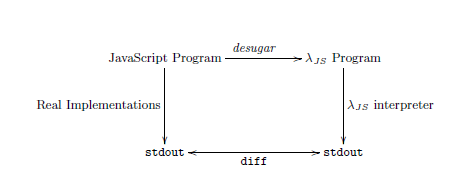
\includegraphics[scale=1]{LambdaJS}
    \caption{The \ljs\ test. Figure taken from \cite{LambdaJS}}
    \label{fig:LJS}
\end{figure}